\documentclass[../IoMusT.tex]{subfiles}
\begin{document}
\subsection{Sistemul de operare Raspbian}
Raspbian este un sistem de operare pentru placa de dezvoltare Rasberry Pi, bazat pe Debian, numele lui venind din combinația cuvintelor Raspberry și Debian. Sunt mai multe versiuni a acestui sistem de perare, ultimul fiind Buster care e compatibil cu toate modelele de Rasperry Pi. Cu toate că a fost creat special pentru acestă placă, este funcțional și pentru sistemele non-Raspberry Pi, fiind dezvoltat pentru arhitecturi de microprocesoare de tip RISC \footnote{Reduced Instruction Set Computer}. Instalarea sistemlui de operație se face relaitv ușor. După descărcarea imaginii și scrierea lui pe card, tot ce trebuie făcut este să butăm placa de dezvoltare. 
\\
\par Dacă utilizăm protocolul Secure Shell pentru a avea acces în sistemul lui Raspberyy Pi, ne dăm seam cu ușurință că sistemul fișierelor eset asemănător cu cel de la sistemul de oprare Linux (mai preic Debian). După butarea plăcii, folderul î care suntem este mereu \verb|/home/pi|. De aici putem naviga în directoarele Desktop șamd. 
\subsection{Protocolul de comunicare MIDI}
\subsubsection{Prezentarea mesajelor MIDI}
% reformulare tastatura
% de completat alte tipuri de mesaje
Comunicarea între un instrument muzical electric și un calculatori se întâmplă de cele mai multe ori printr-un protocol de comunicare numit MIDI (Digital Interface for Musical Interface). Prin acest protocol putem trimite sau primi date de la instrumentul respectiv sub forma unor mesaje MIDI, fiecare astfel de mesaj fiind o instrucțiune. Putem să ne gândim la ele ca fiind o altfel de partitură în care sunt marcate înălțimea și puterea (velocitatea) cu care notele muzicale au fost cântate. Aceste date primite se pot reda audio sau se pot chiar modifica facând acest tip de comunicare un instrument puternic în industria muzicală. 
\\
\par Un mesaj MIDI constă dintr-un octet de stare, care indică tipul mesajului, urmat de până la doi octeți de date care conțin parametrii. Tipul mesajului poate fi de mai multe feluri, acestea variând de la un instrument la altul. Principalele tipuri de mesaje sunt cele de NOTE ON sau NOTE OFF, care indică faptul că interpretul a atins tastatura muzicală respectiv cănd s-a dat drumul la tastă. Diferența de timp dintre aceste două tipuri ne poate da timpul în care a fost ținută o notă muzicală. Cu toate că aceste mesaje sunt unele standard trebuie avut în vedere că nu fiecare instrument poate genera astfel de mesaje. Instrumentele mai vechi au o gamă mai închisă in ceea ce privește multitudinea de tipuri de mesaje ce pot trimite.
\\ 
\par Parametrii unui mesaj MIDI, după cum s-a discutat și în primul paragraf, pot conține nota muzicală și velocitatea cu care aceasta a fost cântată. Reprezentarea acestei note muzicale se face printr-un număr de la 0 pana 127 \cite{MidiSoftware}, 0 fiind nota cea mai joasă cu cea mai mică frecvență. Astfel de exemplu numărul 60 se asociază notei Do cu frecvența 261.63. Puterea cu care nota respectivă a fost apăsată se caracterizează printr-un număr de la 1 la 127 \cite{MidiSoftware}, o apăsare decentă (fără prea multă forță) fiind aproximativ 64. Datorită faptului că pianul folosit în acest proiect are o reprezentare imprecisă a acestui număr, în aplicație ne vom folosi numai numărul notei MIDI din care vom calcula frecvența, folosind o formulă, cu care trebuie să vibreze motoarele când o clapă e apăsată. Când vine vorba despre programarea acestor mesaje, modul în care sunt reprezentate depinde de librăria folosită în limbajul de programare respectiv. Despre parsarea acestora vom detalia în subcapitolele ce urmează.

\subsection{Limbajul de programare Python}
\subsubsection{Prezentare generală}
Python este un limbaj de programare devenit foarte popular datorită faptului că este proiectat să fie ușor de învățat și de înțeles. Este un limbaj de scriptare ceea ce înseamnă că codul scris nu este compilat ci mai degrabă interpretat. Ca și celelalte limbaje de nivel înalt și Python suportă mai multe paradigme de programare cum ar fi programare procedurală, orientată pe obiect sau funcțională sprijinind astfel dezvoltarea unei game largi de aplicații. Poate fi folosit atât pentru realizarea proiectelor de dimensiuni mai mici cât și pentru cele mai mari, fiind cel mai des utilizat în crearea aplicațiilor web (este folosit de companiile Google și Yahoo!), științifice sau de divertisment, cum ar fi jocuri. Este foarte mult folosit și în proiectele ce țin de Internetul lucrurilor, având destule biblioteci ce pot fi folosite pentru programarea senzorilor și actuatorilor.
\\
\par Faptul că limbajul de programare Python oferă o gamă largă de biblioteci și extinderi, constituie un avantaj în programarea aplicațiilor complexe. Biblioteca standard a limbajului este deseori citat și ca unul dintre cele mai mari puncet forte ale sale, oferind multe tool-uri pentru difeite sarcini.
\\
\par Sintaxa și semantica limbajului de programare sunt concepute astfel încât codul să fie cât mai ușor de scris și de înțeles de către programator. Spre deosebire de alte limbaje de programare, Python nu folosește acolade pentru delimitarea blocurilor, aceste delimitări făcându-se cu ajutorul indentării. Un cod indenatat incorect va arunca eroare de tipul IndentationError. Se poate vedea în figura \ref{fig:indent} o bucată de cod indentat corect.
\begin{figure}[h]
\centering
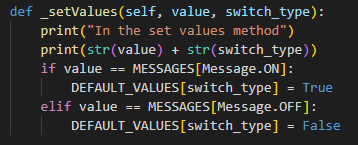
\includegraphics{indentare}
\caption{Exemplu indentare}
\label{fig:indent}
\end{figure}
O scăderii  a indentării  seminfică sfârșitul unui bloc curent în timp ce creșterea indică începerea unei noi afirmații. Un statement (afirmație) este o unitate sintactică a limbajelor de programare imperative care exprimă  unele acțiuni care trebuie efectuate.
\\
\par În Python, ca și în celelalte limbaje de programare, putem face diferența dintre o metodă și o funcție. Ambele trebuie să înceapă cu cuvântul cheie def urmat de denumirea funcției/metodei. Spre deosebire de alte limbaje de programare, în cazul metodelor în Python trebuie specificat explicit cuvântul self în parametrii metodei. Acest cuvânt indică instanța clasei de care aparține metoda respectivă.
% include duck typing

% add cleanup
\subsubsection{Biblioteca Gpiozero pentru programarea pinurilor}
Gpiozero este o bibliotecă care oferă o interfață simplă pentru programarea GPIO-urilor de pe placa de dezvoltare Raspberry Pi. Spre deosebire de alte biblioteci, aceasta oferă o curbă de învățare mai lină pentru începători și posibilitatea dezvoltării proiectelor complicate cu mai multă ușurință și mai puține linii de cod. La început Gpiozero a fost doar un layout peste biblioteca RPi.GPIO, ulterior fiind adăugate diferite suporturi. În prezent RPi.GPIO este folosit ca bibliotecă implicită pentru Gpiozero, această configurație putând fii schimbată, existând ma multe astfel de biblioteci, cum ar fi de exemplu pigpio. Instalarea acestei biblioteci este necesară numai în cazul în care se folosește pe alt sistem de operare decât Raspbian, pe acesta fiind deja inclus. Odată cu instalarea ei putem rula comanda pinout din linia de comandă pentru a vedea vizual detalii despre pinii disponibili de pe Raspberry Pi (vezi figura \ref{fig:pinout}). Acest lucru devine în ajutor în momentul în care, la configurarea pinurilor, trebuie să precizăm numărul pinului ales astfel fiind mult mai ușor de urmat poziționarea fiecărui pin în parte.
\begin{figure}[h]
\centering
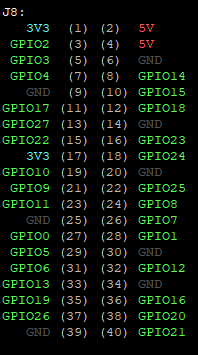
\includegraphics{pinout1}
\caption{Poziționarea pinurilor}
\label{fig:pinout}
\end{figure}
\\
\par În comparație cu alte biblioteci, în Gpiozero se pote observa o abordare orientată pe obiecte, acesta folosind clase în loc de funcții. Pe lângă niște clase specifice, Gpiozero oferă două clase mari de bază, InputDevice și OutputDevice, celelalte fiind derivate din acestea, fiecare având metode și proprietăți specifice care sunt adaptate dispozitivului controlat. Clasa OutputDevices și tot ce derivă din ea este folosită pentru controlarea dispozitivelor de ieșire cum ar fi de exemplu LED-urile, pe când cea de InputDevice este pentru dispozitivele care sunt folosite pentru a furniza date și semnale de control. Asftel alegerea clasei de lucru este mult mai vizibilă și mult mai ușoară.
\\
\par Pentru controlarea motoarelor de vibrații în proiectul de față s-au folosit clasa PWMOutputDevice derivat din OutputDevice care permit și modularea lățimii pulsului. Importarea bibliotecii se face simplu, conform figurei \ref{fig:import}.
\begin{figure}[h]
\centering
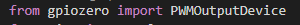
\includegraphics{importPWM}
\caption{Importare biblioteca Gpiozero}
\label{fig:import}
\end{figure}
În momentul instanțierii clasei, în constructor putem da de la unu pana la cinci parametrii, numai primul fiind obligatori, celelalte având deja valorile setate implicit. Parametrul obligatoriu este numărul pinului de pe Raspberry Pi cu care lucrăm. Numerotarea pinurilor în cazul acestei biblioteci se face cu ajutorul sistemului Broadcom. Ceilalți parametrii ai constructorului sunt pentru a seta valoarea de început (duty cycle), frecvența, dacă să fie activ sau nu și nu în ultimul rând putem schimba fabricii de pini, asta fiind o caracteristică avansată pe care majoritatea utilizatorilor o pot ignora. Un exemplu de instanțiere a acestei clase se poate vedea în figura \ref{fig:constructor}, unde parametrul gpio indică numărul pinului setat. .
\begin{figure}[h]
\centering
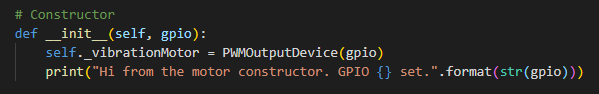
\includegraphics[scale=0.9]{constructorPWM}
\caption{PWMOutputDevice constructor}
\label{fig:constructor}
\end{figure}
\\
%completare ce este duty cycle
\par Datoriă faptului că clasa permite modularea lățimii pulsurilor, se pot seta intensități între valorile 1 și 0, 1 fiind intensitatea maximă cu care motorul poate să vibreze și 0 fiind starea în care se oprește din vibrat. Totodată se poate seta și frecvența, aceasta implicit fiind 100Hz, numărul acesta indicând rata de apariție a unui eveniment repetitiv \cite{Freq}. Exemplu de setare a acestor valori poate fi observat în figura \ref{fig:val}. Clasa dispune mai multe metode și proprietăși cu ajutorul cărora putem porni sau opri dispozitivul. În cazul nostru este deajuns să setăm proprietățile value și frequency pentru a da drumul sau a opri vibrațiile. 
\begin{figure}[h]
\centering
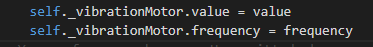
\includegraphics[scale=1.1]{setareValori}
\caption{Setarea valorilor motorului}
\label{fig:val}
\end{figure}
\\
\par Biblioteca Gpiozero pune la dispoziție și o clasă Tone destinată utilizatorilor care folosesc TonalBuzzer pentru a putea reprezenta cu ușurință notele muzicale. Cu toate că în proiectul de față nu este folosit un astfel de dispozitiv, clasa asta ne poate deveni în ajutor la calcularea frecvențelor pornind de la numărul notei MIDI transmis de pian. Datorită faptului că clasa poate fi construită într-o varietate de moduri, asta incluzând și prin numere MIDI, se poate cu ușurință obține frecvența notei respective cu ajutorul atributului frequency. Codul din spatele clasei calculează frecvența cu formula
\[ f = 2^{(d-69)/12} * 440Hz\]
unde parametrul d reprezintă numărul notei muzicale MIDI. Pe lângă nota MIDI, clasa se poate construi pornind și de la frecvență sau de la specificarea notei prin sistemul alfabetic (acesta consistând dintr-o literă majusculă de la A până la G urmat de un modificator opțional și numărul de octave). Folosirea acestei clase se poate vedea în figura \ref{fig:tone}.
\begin{figure}[h]
\centering
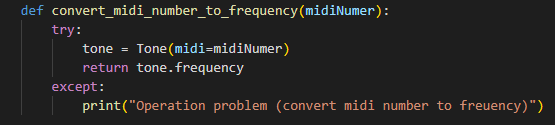
\includegraphics[scale=0.9]{tone}
\caption{Calcularea frecvenței}
\label{fig:tone}
\end{figure}

\subsubsection{Folosirea bibliotecii Mido}
Parsarea și reprezentarea datelor primite de la instrumentul muzical este un pas important în ceea ce privește rularea acestui proiect. Din fericire limbajul de programare Python ne oferă mai multe posibilități prin care putem să ajungem la același rezultat, depinde doar de noi cu ce vrem să lucrăm și care modalitate se potrivește task-ului respectiv. Pentru citirea, parsarea și modificare mesajelor/fișierelor MIDI există mai multe tipuri de biblioteci, fiecare făcând în mare parte același lucru, cu puține diferențe. Biblioteca cu care s-a lucrat în acest proiect se numește Mido și datorită documentației bine pusă la punct este relativ ușor de urmărit ce metode/funcționalități are. Pe parcursul dezvoltării proiectului am încercat să lucrez cu mai multe astfel de tipuri de biblioteci, însă cele mai multe s-au dovedit a fi mai greu de folosit, ducănd lipsă de funcționalități sau având numai metodele minime necesare.
\\
\par Instalarea bibiotecii pe sistemul de operare Raspbian se face cu executarea comenzii pip install mido, iar pentru utilizarea porturilor trebuie instalată și biblioteca rtmidi cu ajutorul comenzii pip install python-rtmidi. Rtmidi este backend-ul folosit în mod implicit care se poate schimba cu altele, cum ar fi PortMidi sau Pygame. Este recomandat să se foloseasă rtmidi din datorită faptului că este mult mai ușor de instalat și are toate caracteristicile celorlalte biblioteci. 
\\
\par Pentru a putea primi date de la pian, trebuie deschis un port de intrare specificând numele portului respectiv (a se vedea figura \ref{fig:port}).
\begin{figure}[h]
\centering
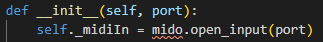
\includegraphics[scale=1.1]{midoPort}
\caption{Port de intrare}
\label{fig:port}
\end{figure}
 Pentru a putea găsi numele portului există metoda \verb|mido.get_input_names()| a bibliotecii, care afișează toate proturile disponibile. Sunt incluse și alte tipuri de porturi în bibliotecă înafară de cele de intrare și de ieșire, precum multi portul care ne permite să citim și să scriem mesaje pe mai multe porturi, SocketPort-ul sau IOPort-ul care este o combinație între cel de intrare și ieșire. După nevoi se pot implementa și altfel de tipuri.
\\
% add 255
\par Mesajele MIDI vor veni pe acest port deschis iar în funcție de arhitectura instrumentului muzical acestea pot veni fără întreruperi, asta însemnând că programul primește date chiar și atunci când nicio o tastă nu a fost apărată pe pian, sau pot veni doar doar când a fost cântată o notă muzicală. În funcție de asta poate fi implementată metoda de parsare a acestor mesaje. În cazul nostru pianul trimite date încontinuu asta însemnând că vor trebui selectate mesajele de care suntem interesate. Iterarea peste mesaje se întâmplă cu ajutorul unui for până când portul se va închide. Pentru o parsare mai ușoară, mesajele de intrare vor fi mai întâi convertate la octeți MIDI ceea ce înseamnă că mai departe se va lucra cu un vector de valori, fiecare valoare corespându-se cu un parametru a notei MIDI respective. Un exemplu de astfel de parsare se poate vedea în figura \ref{fig:midiPars}. 
\begin{figure}[h]
\centering
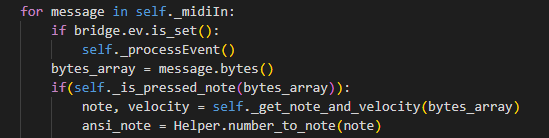
\includegraphics[scale=0.9]{parsareMIDI}
\caption{Citire mesaje MIDI}
\label{fig:midiPars}
\end{figure}
Vectorul găsit conține 3 parametrii printre care ultimele două indică valoarea notei MIDI respectiv puterea cu care acesta a fost cântat/apăsat. Biblioteca mido suportă majoritatea tipurilor de mesaje descrise în prezentarea mesajelor MIDI. 

\subsubsection{Programarea asincrona cu biblioteca Asyncore}
Una dintre metodele cele mai rapide și simple de a trimite mesaje într-o rețetea este comunicare prin sockets. În Python socket-urile sunt obiecte care oferă o modalitate de schimb de informații între două procese între-o manieră directă și independentă de platformă. Aceștia pot fi implementate pe mai multe tipuri de canale diferite cum ar fi TCP\footnote{Transmission Control Protocol} sau UDP\footnote{User Datagram Protocol}. Varianta cea mai de încredere este utilizarea protocolului TCP, care este și cel utilizat în mod implicit, datorită faptului că pachtele aruncate în rețea sunt detectate și retransmise de expeditor și datele sunt citite în ordinea trimiterilor lor. E important să ținem cont de acest lucru datoriă faptului că nu există nicio garanție ca datele trimise să ajungă la destinație. Cele mai comune aplicații cu socket-uri sunt cele de tipuri client-server, unde clientul trimite date către server iar serverul le procesează. Trimiterea acestor mesaje poate fi și una bi-direcțională cum va fi și în cazul nostru. Atât clientul cât și serveril vor trimite date între ele.
\\
\par În limbajul de programare Python aceste socket-uri pot fi implementate cu ajutorul modulului socket, care oferă o interfață de programare a aplicației convenabilă și consistentă. Modul în care aceste socket-uri funcționează este în felul următor: serverul crează un socket, legându-se la o adresă și un port, care va asculat conexiunile de la client la adresa respectovă. Îndată ce un client socket, cu aceeași adresă și port s-a concetat la server se poate începe trimiterea de date. La sfârșit, după ce s-a încheiat tot procesul, clientul poate închide conexiunea cu serverul printr-o simplă metodă \verb|socket.close()|, după care se închide și partea de server.
\\
\par Crearea unui server simplu este ușor de realizat în Python, nefiind atăt de multe metode ce trebuie utilizate. Când vine vorba despre trimiterea datelor către un client la un anumit timp (când sunt disponibile) este mult mai ușor și avantajos de folosit modulul Asyncore, care ne oferă, pe lângă o implementare reactivă a unui socket, posibilitatea de a avea un program asincron ceea ce poate fi un avantaj mare mai ales când avem mai multe socket-uri deschise. Asyncorel ne oferă o infrastructură de bază pentru scrierea socket-urilor de client și server. Astfel programatorul are posibilitatea de a scrie cod care se apelează numai atunci când trebuie să se întâmple ceva (să se trimite sau să se primească anumite date) în loc de a apela metode și de acreea obiecte de tip socket. Ideea de bază în spatele acestui modul este de a crea unul sau mai multe instanțe de clase \verb|asyncore.dispatcher|. Fiecare astfel de canal de rețea creat se adaugă la o hartă globală care eset folosită de funția \verb|loop()|. Apelarea acestei metode \verb|loop()| activează aceste canale, care rulează până când ultimul canal a fost închis.
\\
\par În acest proiect s-au folosit două clase de dispatcher, unul pentru ascultarea socket-ului și unul pentru canalul de client, de unde se vor apela metodele de trimitere și de primire a mesajelor. Implementarea acestor clase se face prin suprascrierea a câtorva metoda care vor manipula acțiunile necesare. Se va apela metoda \verb|handle_accept()| (vezi figura \ref{fig:accept}) când se face o cerere de conectare de la socket-ul client. Aici se va crea o instanță nouă de clasă dispatcher pentru se vor manevra mesajele. Constructorul acestei clase de MessageHandler are ca parametrii un obiect socket care reprezintă conexiunea, adresa clientului conectat și o instanță a clasei de server din care se pornește conexiunea.
\begin{figure}[h]
\centering
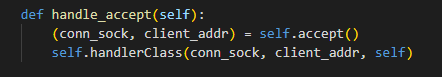
\includegraphics[scale=1.1]{handleAccept}
\caption{Handle accept}
\label{fig:accept}
\end{figure}
\\
\par Pentru trimiterea datelor din serverul de socket către client framework-ul asyncore are implementat o metodă \verb|writable()| care verifică dacă este de trimis un mesaj, acesta implicit returnând True. Suprascrierea acestei metode implică impunerea a unor condiții prin care metoda să verifice dacă chiar este ceva de trimis, atlfel să returneze False. Dacă există date de trimis, framewok-ul va apela automat metoda de \verb|handle_write()| în care eset chemată metoda din modulul socket, \verb|self.send()| (figura \ref{fig:write}).
\begin{figure}[h]
\centering
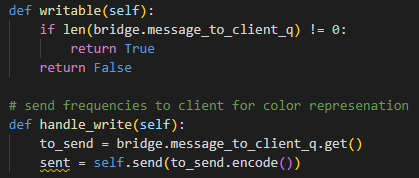
\includegraphics{handleWrite}
\caption{Trimitere date}
\label{fig:write}
\end{figure}
\\
\par Primirea datelor de la client (fie el implementat în Python sau în orice alt limbaj de programare) se face asemănător. Metoda \verb|writable()| determină dacă serverul poate să primească date, iar dacă da, acestea sunt primite și decodate în metoda \verb|handle_read()| (figura \ref{fig:read}. În cazul nostru vream să primim mereu date de la client așa metoda respectivă va returna mereu True.
\begin{figure}[h]
\centering
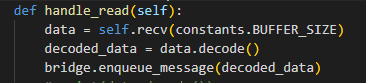
\includegraphics{handleRead}
\caption{Primire date}
\label{fig:read}
\end{figure}

\subsection{Limbajul de programare Java}
\subsubsection{Scurtă introducere}
Limbajul de programare Java este un limbaj cu scop general, bazat pe clasă, orintat pe obiect și proiectat să aibă	cât mai puține dependențe de implementare fiind cel mai popular limbaj de programare în 2019. Sintaxa limbajului seamănă cel mai mult cu cel de C sau C++. Orientarea pe obiect este o caracteristică foarte importantă în ceea ce privește structura acestui limbaj datorită faptului că tot codul scris trebuie să fie într-o clasă. Astfel, în structura unui proiect scris în Java, fiecare fișier reprezintă o clasă separată. Fiecare element de date este un obiect, excepție făcând numai tipurile primitive de date. În comparație cu limbajul de programare C++, Java nu suportă moștenirile multiple și suprascrierea operatorilor.
\\
\par Pentru gestionarea memoriei într-un ciclu de viață a unui obiect Java folosește un colector automat de gunoi\footnote{Garbage collector} care are ca responsabilitate recuperarea memoriei odată ce un obiect nu mai este folosit. Acest lucru se face cu ajutorul referințelor la obiectul respectiv.
\\
\par Limbajul de programare Java este folosit în dezvoltarea a mai multor tipuri de aplicații cum ar fi de exemplu aplicațiile de desktop, mobile, procesare datelor mari\footnote{Big Data} sau de sisteme încorporate. Scopul acestui limaj în proiectul de lincență de față este crearea unei aplicații Android pentru personalizarea experienței utilizatorilor și redarea într-un context vizual sunetele muzicii în ceea ce privește "ascultarea" muzicii de către comunitatea surdă.
\subsubsection{Folosirea firelor de executie in Java}
Firele de execuție joacă un rol important în momentul în care dorim să creăm o aplicație mobilă cu ajutorul limbajului de programare Java. Un fir de execuție poate fi definită ca fiind ce mai mică  unitate de procesare ce poate fi programată spre execuție de către un sistem de operare.Ele permit programelor să facă mai multe lucruri simultan.Acest lucru permite unui utilizator să facă ceva în timp ce altceva se întâmplă pe fundal \cite{articleThread}, firele de execuție execută porțiuni de cod  în paralel în interiorul aceluiași proces. În timp ce comunicarea între procese se poate face numai cu mecanisme de comunicare interprocesare, comunicarea între firele de execuție se întâmplă mult mai ușor și mai rapid, ele având un spațiu de memorie comun și un sistem de semaforizare.
\\
\par Java este un limbaj de programare care are printre principiile sale și suportarea programării pe mai multe fire de execuție. Sistemul Java de rulare depinde de thread-uri datorită a mai multor lucruri. Firele de execuție reduc ineficiența prin prevenirea pierderii ciclirilor  procesorului \cite{Thread}.
\\ 
\par Noțiunea de multithreading înseamnă rularea unei aplicații pe mai multe fire de execuție.În cazul limbajului de programare Java acest sistem este bazat pe clasa \verb|Thread|, pe metodele acestuia și pe interfața \verb|Runnable|. Astfel pentru a crea un firde execuție nou avem două soluții: putem extinde clasa \verb|Thread| și să suprascriem metoda \verb|run()| sau putem să implementăm interfața \verb|Runnable|, ambele având același efect. În interiorul metodei \verb|run()| se va scrie codul care se va executa în dată ce firul de execuție e pornit. Astfel de exemplu se poate vedea în figura \ref{fig:thread}.
\begin{figure}[h]
\centering
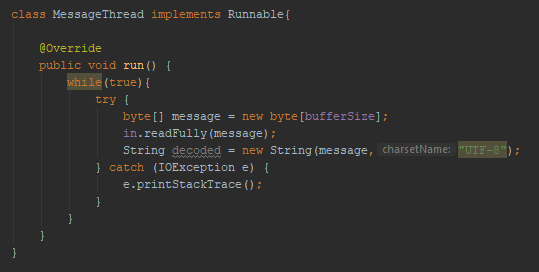
\includegraphics{thread}
\caption{Crearea firelor de execuție}
\label{fig:thread}
\end{figure}
Implementarea acestei metode și crearea unei instanțe a acestei clase nu este deajuns pentru a porni un nou fir de execuție în aplicație. Un fir de execuție are mai multe stări în dealungul vieții lui. Când instanțiem clasa respectivă, îl punem în starea \verb|New|, aceasta indicând că firul de execuție e într-o stare nouă, însă nu se rulează. Rularea unui thread-ului se întâmplă în momentul în care apelăm metoda \verb|start()| pe firul de execuție respectiv, cum se pate vedea și în figura \ref{fig:runthread}. Până atunci acesta va rămâne în starea nouă.
\begin{figure}[h]
\centering
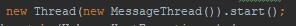
\includegraphics[scale=1.3]{runThread}
\caption{Rularea unui fir de execuție}
\label{fig:runthread}
\end{figure}
\\
%completre ciclu de viata
\par Un fir de execuție poate fi și într-o stare de așteptare ceea ce înseamcă că așteaptă un alt thread să efectueze o sarcină. Acest thread poate să treacă înapoi în starea de rulare numai în cazul în care se semnalează acest lucru.

\subsection{Crearea unei aplicații Android cu Android Studio}
\subsubsection{Sistemul de operare Android}
Android este un sistem de operare care a fost conceput pentru dispozitivele mobile și care inițial a fost dezvoltat de compania Google. Este bazat pe sistemul de operare Linux însă mai multe drivere și biblioteci  au fost modificate sau dezvoltate pentru a permite Android-uli să funcționeze cât mai eficient pe dispozitivele mobile. Aplicațiile Android sunt scrise în limbajul de programare Java și rulate pe o mașină virtuală. Se pot dezvolta aplicații și în limbajul C acestea fiind compilate în cod mașină ARM. Dezvoltarea acestui sistem de operare se întâmplă într-un pas destul de rapid, având un release major nou în fiecare lună  \cite{Android}. Pentru stocarea datelor Android folosește software-ul SQLite
\subsubsection{Android Studio}
Pentru crearea aplicației Android s-a folosit Android Studio datorită faptului că oferă multe funcții care îmbunătățesc productivitatea atunci când vine vorba despre construirea  aplicațiilor Android. Android Studio ne oferă un mediu unificat în care putem dezvolta aplicații pentru toate dispozitivele Android având integrat un emulator rapid cu ajutorul căruia putem testa aplicația fără a conecta un dispozitiv Android la calculator. Emulatorul ne oferă aproape toate capabilitățile unui dispozitiv Android real. Desigur avem posibilitatea de a testa aplicație și pe un telefon real, conectarea acestuia la IDE fiind ușor.
\\
\par Structura unui proiect în Android Studio conține mai multe directoare cu codul sursă atât pentru interfață cât și pentru clasele cu ajutorul cărora aplicația va rula încâ și clasele pentru testarea aplicației. La prima vedere fișierele cele mai importate sunt \verb|AndroidManifest.xml| în care se află codul pentru interfața aplicației, fișierul java \verb|MainActivity| care cel mai bine se poate compara cu funcția \verb|main()| din C++, fiind locul de unde se încarcă componenta UI a aplicației. Dacă avem o aplicație cu ecrane multiple, pentru fiecare ecran o să avem o activitate diferită, activitatea principală fiind fereastra cu care porneșe aplicația. În cazul acestei aplicații vom avea doar o singură fereastră, ciclul acestuia fiind controlată din \verb|MainActivity|. Există și un folder numit res, care conține toate resursele care nu sunt cod cum ar fi machetele XML, șiruri UI și imagini bitmap. Aici putem vedea vizual cum va arăta interfața aplicației fiind și locul în care putem construi UI-ul printr-o simplă tragele a componentelor din paletă.
\subsubsection{Baza de date SQLite}
\end{document}